%%%%%%%%%%%%%%%%%%%%%%%%%%%%%%%%%%%%%%%%%%%%%%%%%%%%%%%%%%%%%%%%%%%%%%%%%%%%%%%

\chapter{INTRODUÇÃO}

O conjunto de Cantor $\mathcal{C}$ é um subconjunto do intervalo [0,1] definido pelo matemático George Cantor no paper \citeonline{cantor1884puissance}. Esse conjunto é obtido a partir de repetidas remoções do terço médio de um segmento. Iniciando com o intervalo fechado $[0,1]$, remove-se o intervalo aberto $(\frac{1}{3},\frac{2}{3})$ para se obter $[0,\frac{1}{3}] \bigcup [\frac{2}{3}, 1]$, que são dois segmentos fechados disjuntos. No próximo passo, os terços médios destes dois segmentos são removidos gerando assim quatro segmentos. O conjunto de Cantor é o resultado desta operação após infinitos passos (ver Figura \ref{fig:fractal}).

\begin{figure}[ht!]
	\vspace{1mm}	% acrescentar o espaçamento vertical apropriado entre o título e a borda superior da figura
	\begin{center}
		\resizebox{15cm}{!}{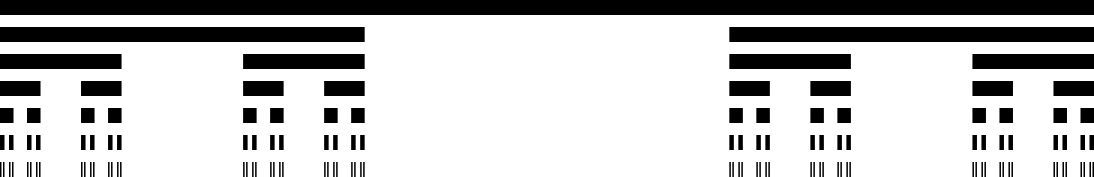
\includegraphics{../Figuras/cantor_fractal.png}}
	\end{center}
	\vspace{1mm}	% acrescentar o espaçamento vertical apropriado entre a borda inferior da figura e a legenda ou a fonte quando não há legenda (o valor pode ser negativo para subir)
	\caption{Conjunto de Cantor após sete iterações. FONTE: en.wikipedia.org Image:Cantor\_set\_in\_seven\_iterations.svg.}
	%\legenda{LEGENDA.} % 	% legenda - para deixar sem legenda usar comando \legenda{} (nunca deve-se comentar o comando \legenda)
	\label{fig:fractal}
	%\FONTE{}	% fonte consultada (elemento obrigatório, mesmo que seja produção do próprio autor)
\end{figure}

O conjunto $\mathcal{C}$ é um conjunto compacto e não vazio. Seja $\mathcal{C}_{0} = [0,1]$ e $\mathcal{C}_{1} = \mathcal{C}_{0}- (\frac{1}{3},\frac{2}{3})$, e seja $\mathcal{C}_{n}$ o resultado após $n$ passos. Portanto, o conjunto de Cantor pode ser escrito como $\mathcal{C} = \bigcap_{n=0}^{\infty} \mathcal{C}_{n}$. Cada conjunto $\mathcal{C}_{n}$ é a união de conjunto finitos compactos e é portanto compacto. Além disso, $\mathcal{C}_{n+1} \subset \mathcal{C}_{n}$ para todo $n$, portanto $\mathcal{C}_{n}$ é a interseção de conjuntos compactos cada vez menores.

Outras propriedades do conjunto de Cantor são: tem tamanho infinito e não numerável, é um fractal e tem medida nula. Por sua vez, a \textbf{função de Cantor} $G$, também função de Lebesgue ou escadaria do diabo, é uma função com as seguintes propriedades \cite{dovgoshey2006cantor}: 
\begin{itemize}
\item $G$ é contínua e crescente mas não absolutamente contínua.
\item $G$ é uma função singular.
\item $G$ mapeia o conjunto de Cantor $\mathcal{C}$ no intervalo [0,1].
\end{itemize}

Essa função é muito interessante de ser estudada no contexto da análise de sinais. De forte variação e não estacionária, ela pode ser explorada a partir da Transformada Janelada de Fourier. O presente estudo testa diferentes funções janela e produz espectrogramas da função de Cantor para diferentes valores de $n$ do conjunto $\mathcal{C}_{n}$. Este manuscrito está assim dividido: na Seção 2 a metodologia empregada é apresentada; na Seção 3 os resultados são oferecidos com breve discussão; na Seção 4 estão as considerações finais do autor.





